\documentclass[border=6pt]{standalone}
\usepackage{tikz}
\usetikzlibrary{arrows.meta,positioning,calc,fit,backgrounds}

\begin{document}
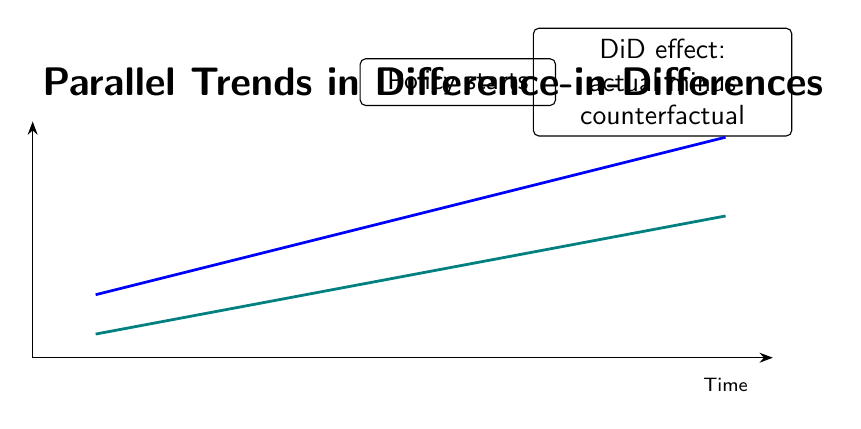
\begin{tikzpicture}[
  font=\sffamily,
  >=Stealth,
  title/.style={font=\sffamily\bfseries\Large},
  explainer/.style={draw, rounded corners=2pt, align=center, inner sep=4pt},
  lab/.style={font=\sffamily\scriptsize, align=center}
]
\node[title, anchor=west] at (0,3.5) {Parallel Trends in Difference-in-Differences};
\node[explainer, text width=2.2cm] at (5.4,3.5) {Policy starts};
\node[explainer, text width=3.0cm] at (8.0,3.5) {DiD effect: actual minus counterfactual};
\draw[->] (0,0) -- (9.4,0);
\draw[->] (0,0) -- (0,3.0);
\draw[blue, line width=1pt] (0.8,0.8) -- (8.8,2.8);
\draw[teal, line width=1pt] (0.8,0.3) -- (8.8,1.8);
\node[lab] at (8.8,-0.35) {Time};
\end{tikzpicture}
\end{document}
